\section{External Validation in the University Hospital Erlangen Cohort}
\label{sec:external-validation}

\subsection{Purpose and validation design}
\label{sec:external-validation:scope}

Section~\ref{sec:reference} reproduced the diagnostic and prognostic models of
the reference study \citep{Li2023} using data from the Surveillance, Epidemiology, and End
Results (SEER) programme. This section evaluates whether those models retain
predictive value in an independent hospital cohort from University Hospital
Erlangen (\emph{Universit\"atsklinikum Erlangen}, abbreviated as UK Erlangen).
The cohort contains 30 patients and was not used to develop or select any of the
models. This analysis concerns only the conventional reference-study models; it
does not validate the foundation-model, embedding, multilayer-perceptron or
synthetic-data experiments presented later in the report.

All model components were kept unchanged during external validation. In this
report, an unchanged or ``frozen'' model means that its predictors, coefficients,
categorical definitions and decision rules were taken directly from the SEER
reproduction. No model was refitted, no variable was reselected, no predicted
probability was recalibrated and no threshold was chosen using the Erlangen
patients. The diagnostic analysis evaluates the 5-variable logistic-regression
nomogram as the primary model. The 6-variable specification described in the
reference-study text, the 8-variable data-driven reproduction and a comparator
using tumour (T) and nodal (N) stage were also evaluated. The prognostic analysis
evaluates the 5-variable Cox proportional-hazards nomogram as the primary model
and compares it with a Cox model containing only T and N stage. This design
assesses how the SEER-trained models perform in a different clinical population,
without adapting them to the small external cohort.

\subsection{Cohort composition}
\label{sec:external-validation:cohort}

The external dataset contained 30 unique patients. All 30 entered the diagnostic
cohort: 11 (36.7\%) had liver metastasis at diagnosis and 19 did not. The same 11
liver-metastasis-positive patients formed the prognostic cohort; 7 died during
follow-up and 4 were censored, meaning that follow-up ended before death was
observed. Table~\ref{tab:external-validation:cohort} summarises the main cohort
characteristics. Continuous variables are reported as median [first quartile,
third quartile], and categorical variables as count (percentage). Exact tumour
diameter was available for 26 diagnostic patients and 8 prognostic patients. One
patient had missing N stage. Marital status was unknown for 11 diagnostic
patients, including 2 patients in the prognostic cohort.

\begin{table}[htbp]
\centering\small
\caption{Characteristics of the University Hospital Erlangen external cohort.
The prognostic cohort is the liver-metastasis-positive subset of the diagnostic
cohort. Percentages use the full cohort size as the denominator; consequently,
the N1 percentages include the patient with missing N stage in the denominator.
Tumour-size summaries include only patients with an exact measurement in
millimetres.}
\label{tab:external-validation:cohort}
\begin{tabularx}{\linewidth}{@{}Yrr@{}}
\toprule
Characteristic & Diagnostic cohort & Prognostic subset \\
\midrule
\csname @@input\endcsname{tables/external_validation/cohort_summary_rows.tex}
\bottomrule
\end{tabularx}
\end{table}

The external cohort differed from the SEER cohorts used for model development.
Liver metastasis was present in 36.7\% of the Erlangen diagnostic cohort compared
with 17.3\% of the SEER diagnostic cohort. Within the Erlangen prognostic cohort,
5 of 11 patients had T4 disease and only 1 underwent primary-tumour surgery. The
different case mix provides a meaningful test of whether the model predictions
transfer to another setting. However, the small number of patients limits the
precision of every estimate and does not support reliable subgroup comparisons.

\subsection{Data harmonisation and model compatibility}
\label{sec:external-validation:mapping}

The Erlangen variables were converted to the same definitions, units and
categories used to train the SEER models. Patient identifiers were replaced with
project-specific pseudonyms, and only aggregate results are presented in this
report. Sex and explicit yes/no variables were converted to binary indicators.
Histological grades I--IV were represented as values 1--4. Morphology codes from
the International Classification of Diseases for Oncology, Third Edition
(ICD-O-3), were mapped to the detailed diagnostic categories and to the broader
carcinoid-versus-other grouping required by the prognostic model. Primary
pancreatic site was grouped as head, body, tail or other. Tumour and nodal stages
followed the categories of the American Joint Committee on Cancer (AJCC) and were
retained as categorical variables.

Exact tumour diameters were grouped as 0--26~mm, 26--36~mm or greater than
36~mm, matching the SEER model definitions. When a tumour size was reported only
as a bound, such as less than 20~mm or greater than 40~mm, the bound was used to
assign the valid size category but was not replaced by an invented exact value.
Unknown marital status and missing N stage were likewise retained as missing
rather than assigned to an observed category.

After recoding, the data were checked for unique patients, valid categories,
compatible units and correct restriction of the prognostic analysis to patients
with liver metastasis. All observed categories were compatible with the fitted
models. Because the analyses used complete cases for the predictors required by
each model, the evaluable sample varied slightly. The 4 diagnostic models shared
a common set of 29 patients because 1 patient lacked N stage. The primary
prognostic nomogram could be applied to all 11 patients, whereas the comparison
with the T/N-stage model used 10 patients. Supplementary prognostic models that
also required marital status could be applied to only 8 patients. These
differences arise from missing predictor values, not from errors in recoding.

\subsection{Evaluation methods and uncertainty}
\label{sec:external-validation:methods}

Diagnostic discrimination was measured with the area under the receiver
operating characteristic curve (AUC). An AUC of 0.5 represents chance-level
ranking, whereas 1.0 represents perfect separation of patients with and without
liver metastasis. Overall probability error was measured with the Brier score,
for which lower values indicate more accurate probabilities. Calibration was
assessed with calibration-in-the-large and calibration slope. Their ideal values
are 0 and 1, respectively. Decision-curve analysis compared the models' net
benefit across possible risk thresholds.

Prognostic discrimination was assessed with Harrell's concordance index
(C-index) and with cumulative/dynamic AUC at 12, 24 and 36 months. The C-index
measures whether patients assigned higher risk tend to experience death earlier.
The time-specific AUC measures discrimination between patients who died by a
given time and those who remained event-free beyond that time, while accounting
for censoring. Prediction error at each time point was measured with a Brier
score using inverse probability of censoring weighting (IPCW). Observed survival
was estimated with the Kaplan--Meier method and compared with the mean survival
predicted by the model.

Uncertainty was estimated with 5,000 patient-level bootstrap resamples. The same
resampled patients were used across models within each task to make comparisons
as consistent as possible. Diagnostic resampling preserved the numbers of
patients with and without liver metastasis. Reported intervals are percentile
95\% confidence intervals for performance of the already fitted models in this
external sample. They do not include uncertainty from the earlier SEER variable
selection or model-development process.

\subsection{Diagnostic external validation}
\label{sec:external-validation:diagnostic}

All 3 multivariable diagnostic models showed strong discrimination in the common
29-patient set (Table~\ref{tab:external-validation:diagnostic}). The primary
5-variable nomogram achieved an AUC of 0.934 (95\% confidence interval
0.809--1.000), and the 8-variable data-driven model achieved 0.942
(0.837--1.000). The T/N-stage comparator achieved 0.739 (0.521--0.927). The wide,
overlapping intervals do not support a precise ranking of the 3 multivariable
models. Brier scores were approximately 0.10 for those models and 0.189 for the
T/N-stage comparator.

\begin{table}[htbp]
\centering\scriptsize
\setlength{\tabcolsep}{3pt}
\caption{Diagnostic performance in the 29 patients with all predictors required
by the 4 models. Values in parentheses are 95\% patient-bootstrap confidence
intervals. Calibration-in-the-large (CITL) compares the overall observed event
frequency with the model predictions; ideal CITL is 0 and ideal calibration
slope is 1.}
\label{tab:external-validation:diagnostic}
\begin{tabularx}{\linewidth}{@{}p{3.15cm}rYYYY@{}}
\toprule
Model & $n$ & AUC & Brier score & CITL & Calibration slope \\
\midrule
\csname @@input\endcsname{tables/external_validation/diagnostic_results_rows.tex}
\bottomrule
\end{tabularx}
\end{table}

For the primary nomogram, the positive CITL indicates that the observed frequency
of liver metastasis was higher than the model predicted on average. Its
calibration slope above 1 indicates that the predicted risks varied less across
patients than the observed outcomes supported. The 6-variable reference-text
model was closer to the ideal calibration values by point estimate, but its
confidence intervals were also broad. The grouped calibration plot and decision
curves in Figure~\ref{fig:external-validation:diagnostic} are therefore
descriptive. With only 10 patients with liver metastasis in the common analysis
set, they cannot identify a stable risk threshold or establish clinical benefit.

\begin{figure}[htbp]
\centering
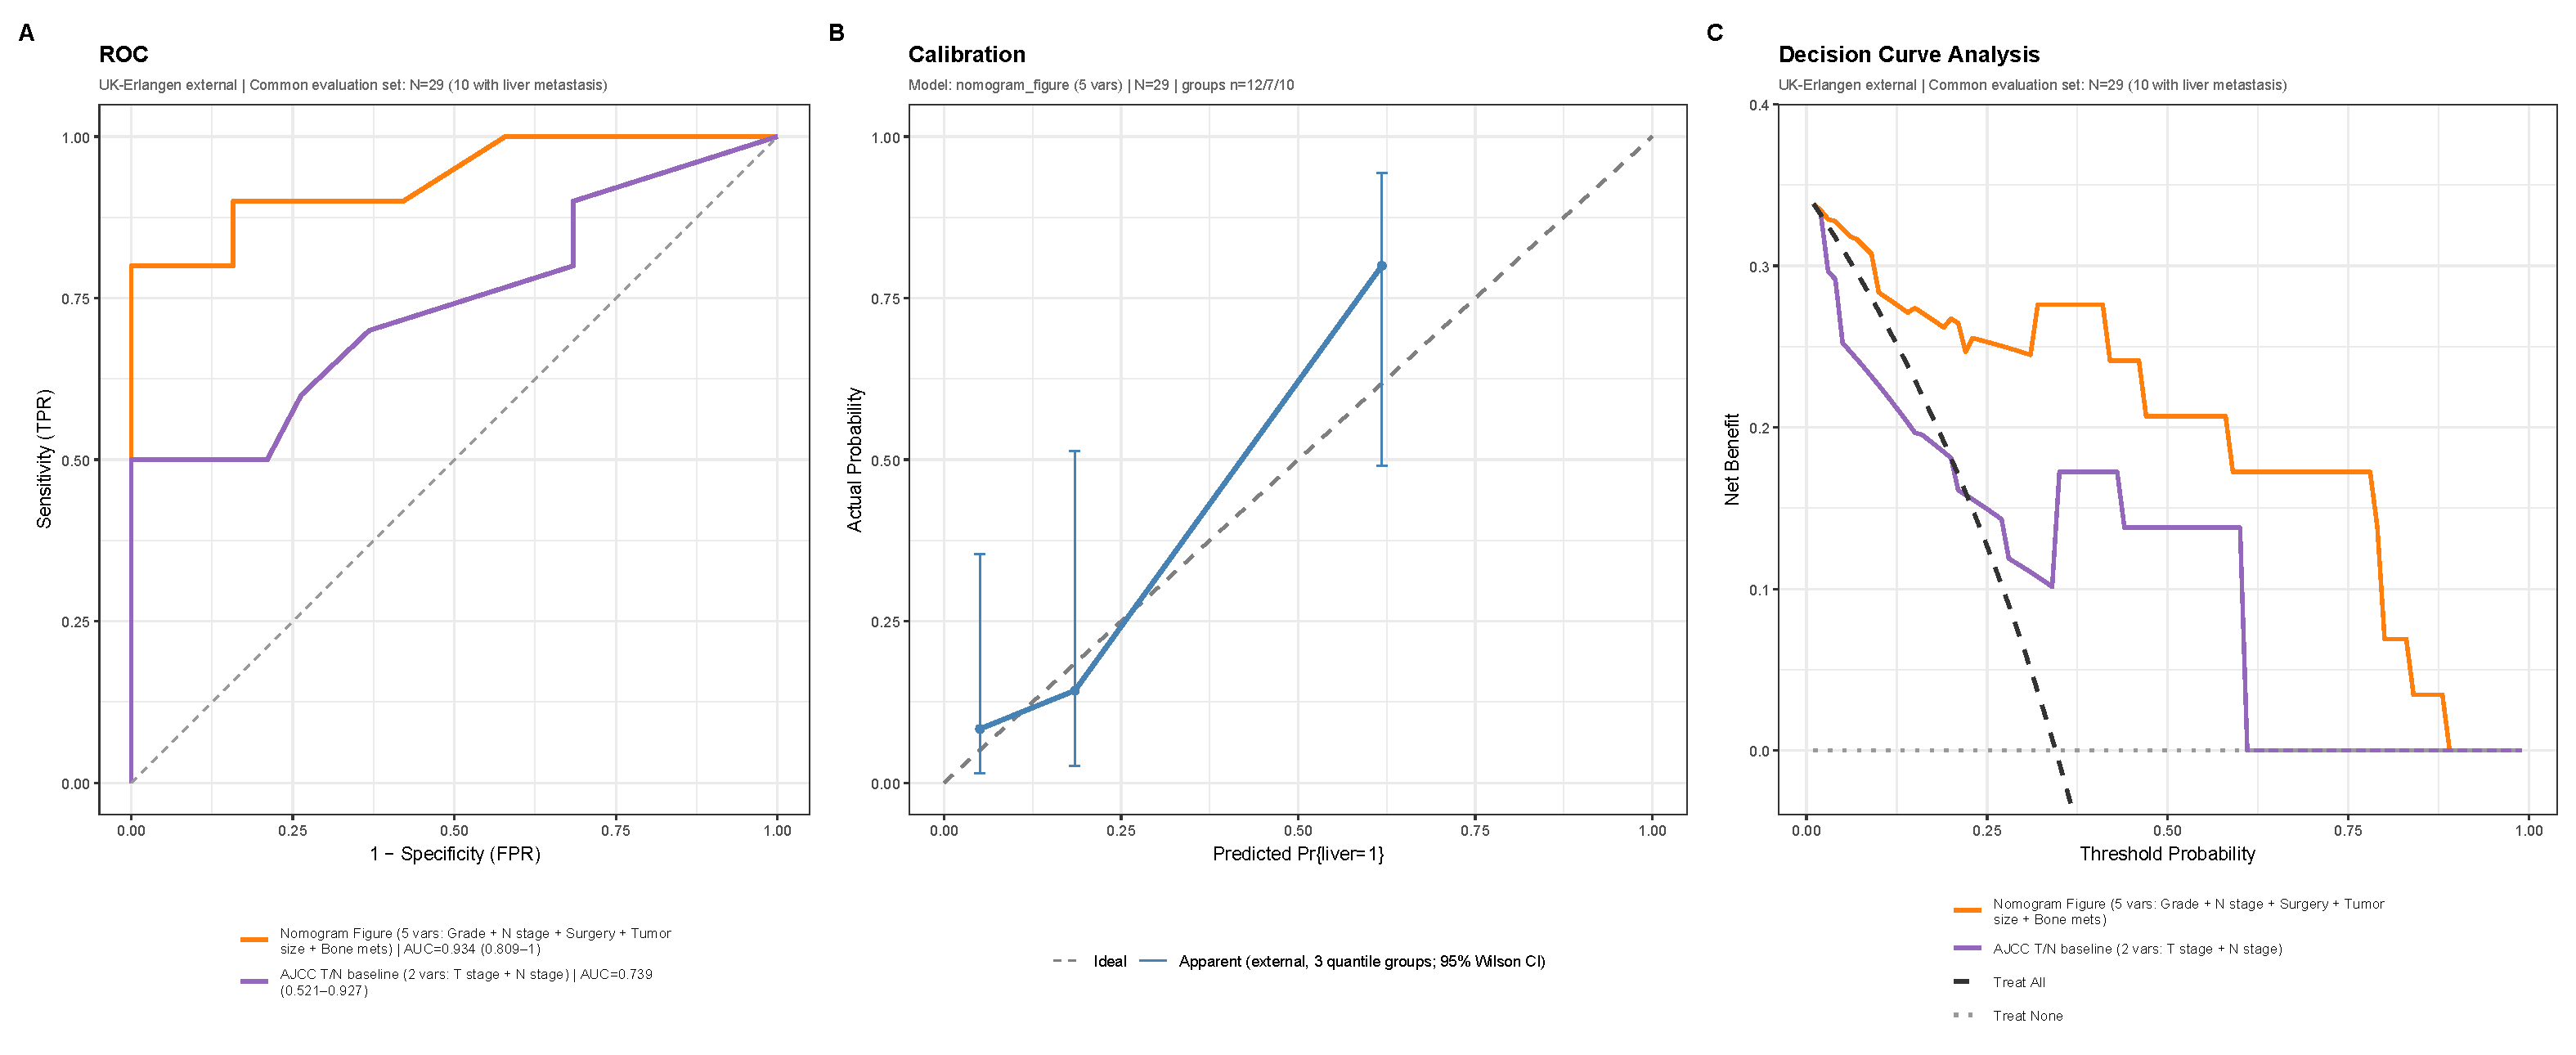
\includegraphics[width=\linewidth]{external_validation/diagnostic_external_evaluation_3panel.pdf}
\caption{Diagnostic external validation in the common 29-patient set: receiver
operating characteristic curves (A), calibration across 3 predicted-risk groups
(B) and decision-curve analysis (C). The models were trained on the reproduced
SEER cohort and applied without modification. The curves are imprecise because
the common set contains only 10 patients with liver metastasis.}
\label{fig:external-validation:diagnostic}
\end{figure}
\FloatBarrier

\subsection{Prognostic external validation}
\label{sec:external-validation:prognostic}

The primary 5-variable prognostic nomogram---containing brain metastasis, age,
grade, histological group and primary-tumour surgery---could be evaluated in all
11 liver-metastasis-positive patients. Its C-index was 0.833 (95\% confidence
interval 0.625--1.000). In the common 10-patient set, the nomogram's C-index was
0.824 compared with 0.676 for the T/N-stage model
(Table~\ref{tab:external-validation:prognostic-discrimination}). The nomogram's
AUC estimates were 0.954 at 12 months, 0.936 at 24 months and 0.833 at 36 months
when all 11 eligible patients were used. All confidence intervals were wide. The
T/N-stage model's AUC also changed considerably across time points, reflecting
the very small numbers of deaths and surviving patients available at each time
rather than reliable evidence of superior performance at 36 months.

\begin{table}[htbp]
\centering\scriptsize
\setlength{\tabcolsep}{3pt}
\caption{External prognostic discrimination for the SEER-trained 5-variable
nomogram and the T/N-stage comparator. The first row uses all 11 patients
evaluable for the nomogram; the remaining rows use the same 10 patients for both
models. Values in parentheses are 95\% patient-bootstrap confidence intervals.}
\label{tab:external-validation:prognostic-discrimination}
\begin{tabularx}{\linewidth}{@{}p{3.0cm}rrYYYY@{}}
\toprule
Model and evaluation set & $n$ & Deaths & C-index & AUC$_{12}$ & AUC$_{24}$ & AUC$_{36}$ \\
\midrule
\csname @@input\endcsname{tables/external_validation/prognostic_discrimination_rows.tex}
\bottomrule
\end{tabularx}
\end{table}

\begin{figure}[htbp]
\centering
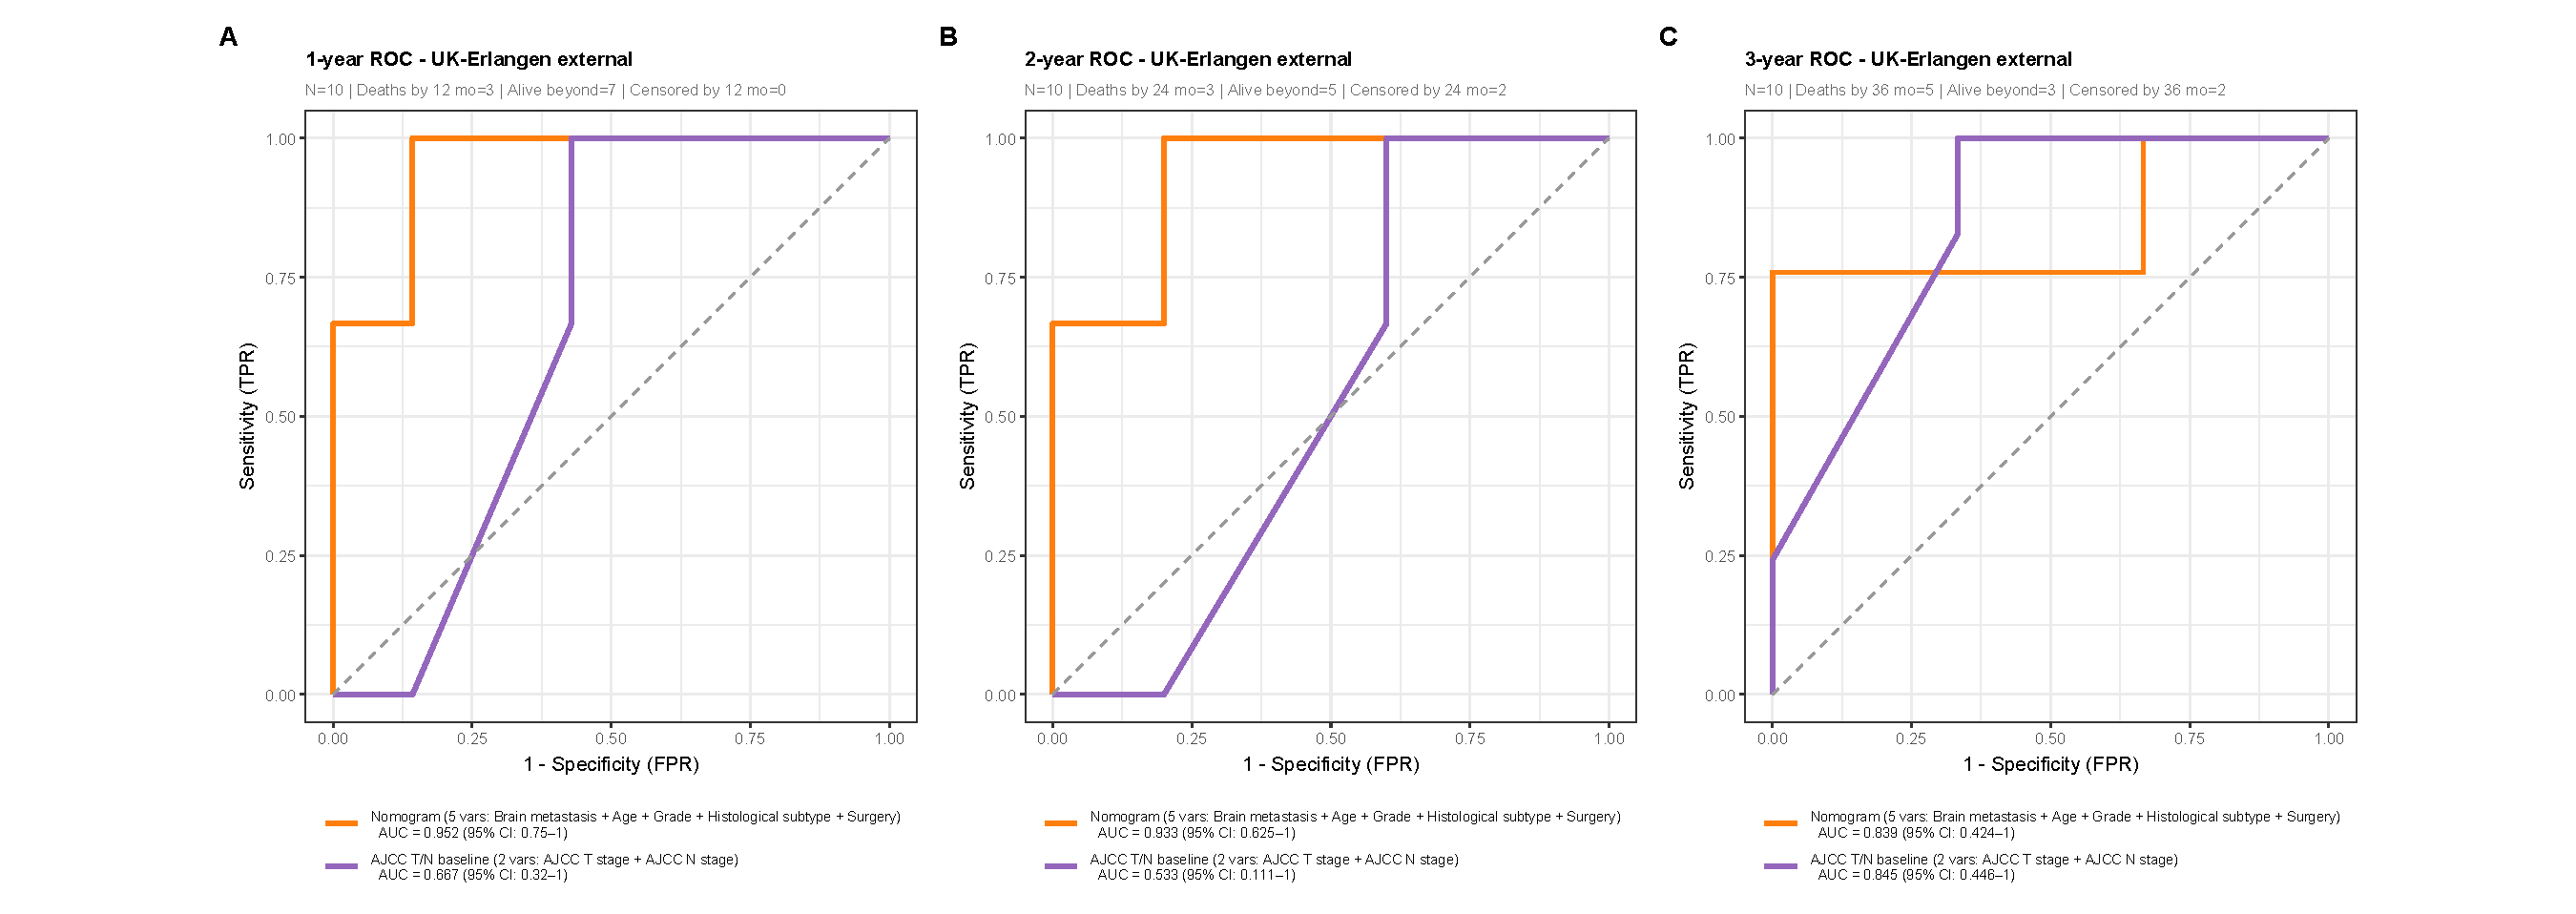
\includegraphics[width=\linewidth]{external_validation/prognostic_external_time_roc_3panel.pdf}
\caption{Time-specific receiver operating characteristic curves at 12, 24 and
36 months for the prognostic nomogram and T/N-stage model in their common
10-patient set. Only 3 deaths occurred by 12 and 24 months and 5 by 36 months, so
the estimates are highly discrete and imprecise.}
\label{fig:external-validation:prognostic-roc}
\end{figure}

For the primary nomogram, the IPCW Brier scores were 0.116, 0.123 and 0.153 at
12, 24 and 36 months, respectively
(Table~\ref{tab:external-validation:prognostic-calibration}). The difference
between Kaplan--Meier observed survival and mean predicted survival was 0.013 at
12 months, 0.139 at 24 months and $-0.030$ at 36 months. Every confidence interval
included 0 and was too wide to demonstrate close agreement between observed and
predicted survival. Figure~\ref{fig:external-validation:prognostic-calibration}
also displays calibration within 3 predicted-risk groups. Each group contains
only 3 or 4 patients, so these group-level estimates are exploratory. Prognostic
decision curves are not shown because the cohort did not meet the prespecified
minimum of 20 evaluable patients and 5 deaths at a given time point.

\begin{table}[htbp]
\centering\scriptsize
\caption{Prediction error and calibration of the primary 5-variable prognostic
nomogram in all 11 eligible patients. The calibration gap is Kaplan--Meier
observed survival minus mean predicted survival; 0 indicates agreement. Values
in parentheses are 95\% patient-bootstrap confidence intervals.}
\label{tab:external-validation:prognostic-calibration}
\begin{tabularx}{\linewidth}{@{}r r Y Y Y Y@{}}
\toprule
Months & $n$ & IPCW Brier & Kaplan--Meier survival & Mean predicted survival & Calibration gap \\
\midrule
\csname @@input\endcsname{tables/external_validation/prognostic_calibration_rows.tex}
\bottomrule
\end{tabularx}
\end{table}

\begin{figure}[htbp]
\centering
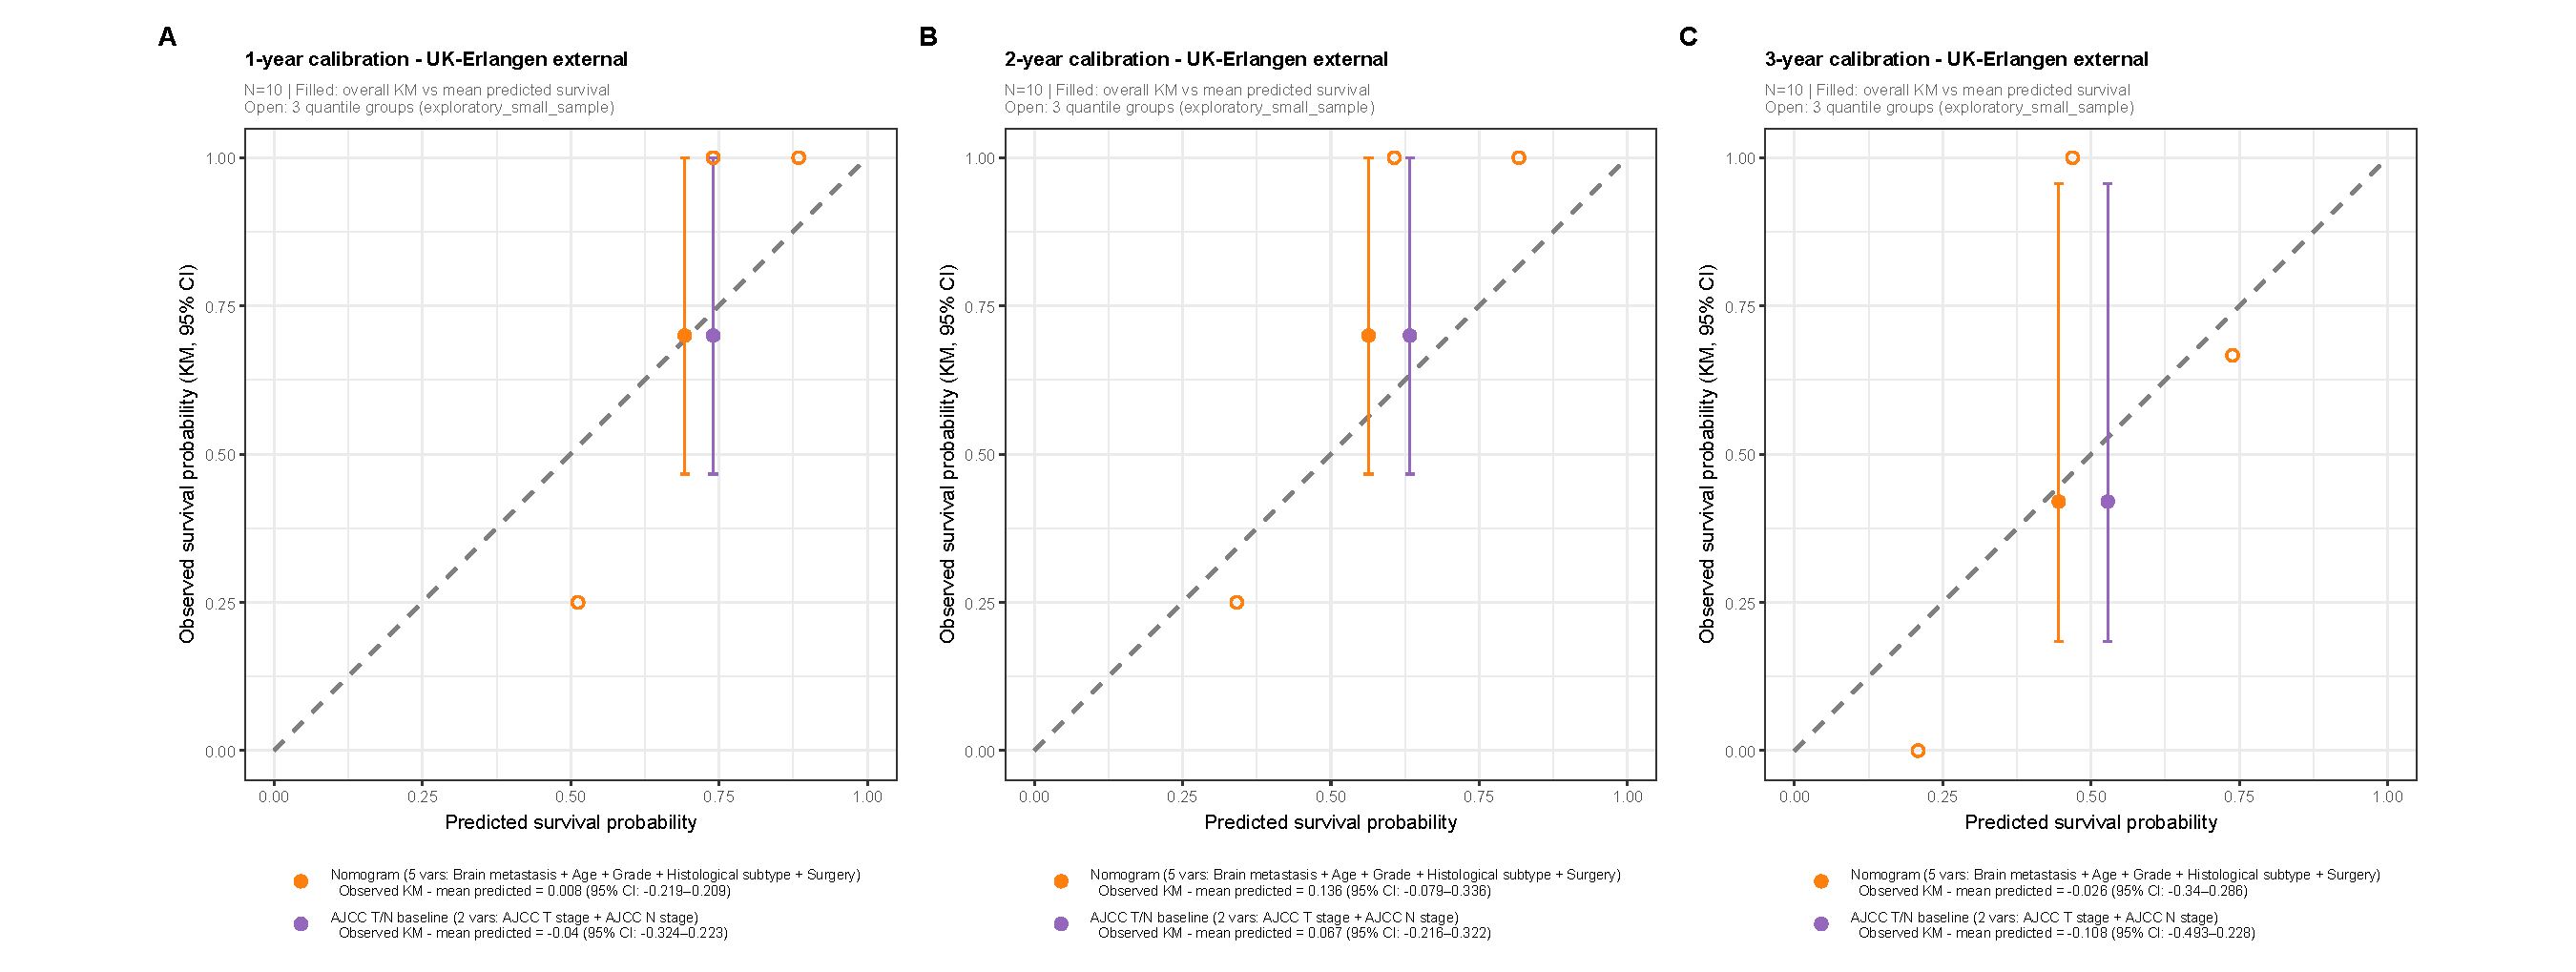
\includegraphics[width=\linewidth]{external_validation/prognostic_external_calibration_3panel.pdf}
\caption{Calibration of the primary 5-variable prognostic nomogram at 12, 24 and
36 months in all 11 eligible patients. Filled points compare overall
Kaplan--Meier survival with mean predicted survival; open points show the
exploratory estimates for 3 predicted-risk groups. Wide confidence intervals and
estimates at 0 or 1 reflect the very small group sizes.}
\label{fig:external-validation:prognostic-calibration}
\end{figure}

The prognostic nomogram's risk cutpoint of 0.232769 was derived from the SEER
training cohort and applied unchanged. It assigned 4 Erlangen patients to the
low-risk group and 7 to the high-risk group. Median overall survival was 44
months in the low-risk group and 29 months in the high-risk group; the log-rank
test gave $p=0.191$. In Figure~\ref{fig:external-validation:km}, the high-risk
curve reaches 0 when the last patient at risk dies at 47 months. The low-risk
curve remains flat at later times because 1 censored patient was followed for 199
months. These are valid Kaplan--Meier estimates for the observed patients, but
the 2 small groups do not support stable estimates of population survival.

\begin{figure}[htbp]
\centering
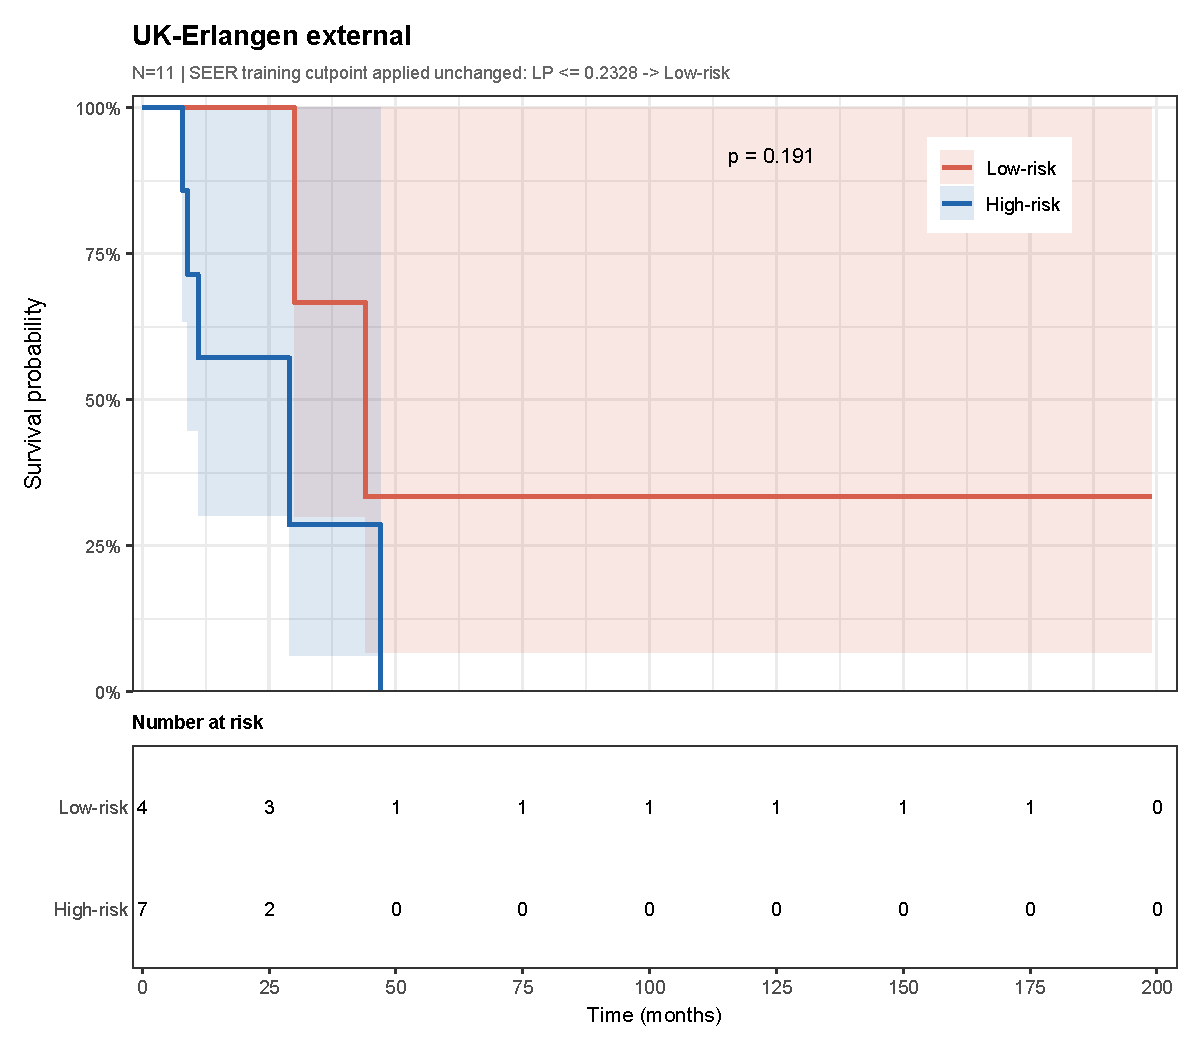
\includegraphics[width=0.74\linewidth]{external_validation/prognostic_external_km_risk_groups.pdf}
\caption{Kaplan--Meier survival after applying the unchanged SEER-derived risk
cutpoint to the primary 5-variable prognostic nomogram. Shading shows pointwise
95\% confidence intervals, and the lower panel gives the number of patients
remaining at risk. The groups contain only 4 and 7 patients; therefore, the
non-significant log-rank result is inconclusive and does not demonstrate equal
survival.}
\label{fig:external-validation:km}
\end{figure}
\FloatBarrier

\subsection{Interpretation and transition}
\label{sec:external-validation:interpretation}

The independent Erlangen cohort shows that the SEER-trained diagnostic models
retained strong ability to rank patients by the presence of liver metastasis.
The primary prognostic nomogram also ranked survival outcomes better than the
T/N-stage comparator by point estimate. These findings are encouraging, but the
wide confidence intervals show that the exact performance values remain
uncertain.

The calibration and decision-curve results require greater caution. The cohort
contains only 30 patients for diagnosis and 11 for prognosis, and several
analyses use even fewer complete cases. It is therefore not possible to make
reliable claims about clinical benefit, performance in patient subgroups or
readiness for clinical deployment. The results support the technical
applicability of the unchanged SEER models to the available Erlangen data, while
also showing the need for validation in a substantially larger independent
cohort.

This section validates only the diagnostic and prognostic models reproduced from
the reference study. The next section returns to the SEER data and introduces
the Tabular Prior-Data Fitted Network (TabPFN) representations and the generation
of synthetic cohorts containing both predictors and outcomes for the subsequent
experiments.
\FloatBarrier
